\documentclass[tikz,border=2pt]{standalone}
\usepackage{tikz}

\begin{document}
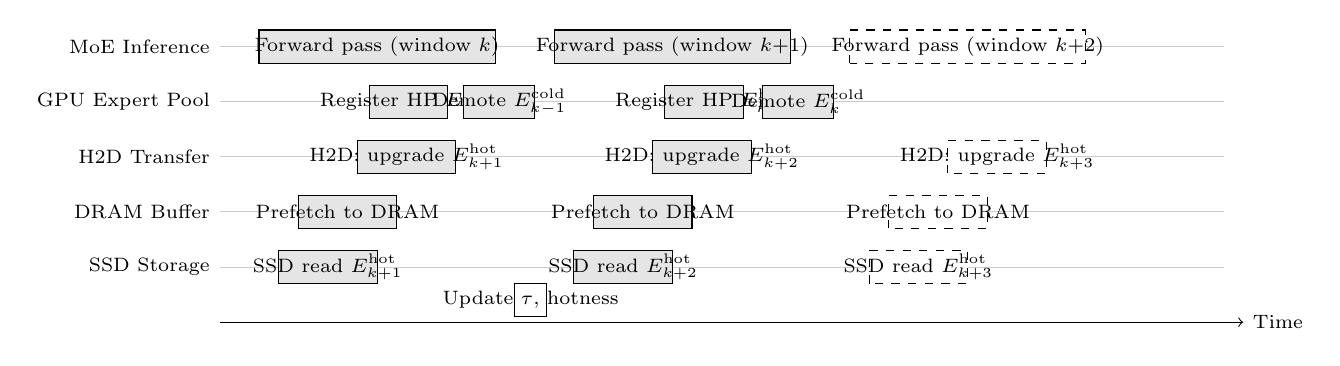
\begin{tikzpicture}[x=0.5cm,y=0.7cm,font=\scriptsize]
      % Axes
      \draw[->] (0,0) -- (26,0) node[anchor=west] {Time};

      % Lane labels
      \node[anchor=east] at (0,5) {MoE Inference};
      \node[anchor=east] at (0,4) {GPU Expert Pool};
      \node[anchor=east] at (0,3) {H2D Transfer};
      \node[anchor=east] at (0,2) {DRAM Buffer};
      \node[anchor=east] at (0,1) {SSD Storage};
      %\node[anchor=east] at (0,0.2) {Controller};

      % Horizontal lane lines
      \draw[gray!40] (0,5) -- (25.5,5);
      \draw[gray!40] (0,4) -- (25.5,4);
      \draw[gray!40] (0,3) -- (25.5,3);
      \draw[gray!40] (0,2) -- (25.5,2);
      \draw[gray!40] (0,1) -- (25.5,1);

      % ==== Window k ====
      % Forward pass (window k)
      \draw[fill=black!10,draw=black] (1,4.7) rectangle (7,5.3);
      \node at (4,5) {Forward pass (window $k$)};

      % SSD -> DRAM prefetch for k+1
      \draw[fill=black!10,draw=black] (1.5,0.7) rectangle (4.0,1.3);
      \node at (2.75,1) {SSD read $E^{\mathrm{hot}}_{k+1}$};

      \draw[fill=black!10,draw=black] (2.0,1.7) rectangle (4.5,2.3);
      \node at (3.25,2) {Prefetch to DRAM};

      % DRAM -> GPU memory upgrade for k+1
      \draw[fill=black!10,draw=black] (3.5,2.7) rectangle (6.0,3.3);
      \node at (4.75,3) {H2D: upgrade $E^{\mathrm{hot}}_{k+1}$};

      % GPU memory pool changes
      \draw[fill=black!10,draw=black] (3.8,3.7) rectangle (5.8,4.3);
      \node at (4.8,4) {Register HP $E^{\mathrm{hot}}_{k+1}$};

      % Demote old experts (k-1)
      \draw[fill=black!10,draw=black] (6.2,3.7) rectangle (8.0,4.3);
      \node at (7.1,4) {Demote $E^{\mathrm{cold}}_{k-1}$};

      % ==== Window k+1 ====
      % Forward pass (window k+1)
      \draw[fill=black!10,draw=black] (8.5,4.7) rectangle (14.5,5.3);
      \node at (11.5,5) {Forward pass (window $k{+}1$)};

      % SSD -> DRAM prefetch for k+2
      \draw[fill=black!10,draw=black] (9.0,0.7) rectangle (11.5,1.3);
      \node at (10.25,1) {SSD read $E^{\mathrm{hot}}_{k+2}$};

      \draw[fill=black!10,draw=black] (9.5,1.7) rectangle (12.0,2.3);
      \node at (10.75,2) {Prefetch to DRAM};

      % DRAM -> GPU memory upgrade for k+2
      \draw[fill=black!10,draw=black] (11.0,2.7) rectangle (13.5,3.3);
      \node at (12.25,3) {H2D: upgrade $E^{\mathrm{hot}}_{k+2}$};

      % GPU memory pool changes
      \draw[fill=black!10,draw=black] (11.3,3.7) rectangle (13.3,4.3);
      \node at (12.3,4) {Register HP $E^{\mathrm{hot}}_{k+2}$};

      \draw[fill=black!10,draw=black] (13.8,3.7) rectangle (15.6,4.3);
      \node at (14.7,4) {Demote $E^{\mathrm{cold}}_{k}$};

      % ==== Window k+2 (illustrative, dashed) ====
      \draw[fill=white,draw=black,dashed] (16.0,4.7) rectangle (22.0,5.3);
      \node at (19.0,5) {Forward pass (window $k{+}2$)};

      \draw[fill=white,draw=black,dashed] (16.5,0.7) rectangle (19.0,1.3);
      \node at (17.75,1) {SSD read $E^{\mathrm{hot}}_{k+3}$};

      \draw[fill=white,draw=black,dashed] (17.0,1.7) rectangle (19.5,2.3);
      \node at (18.25,2) {Prefetch to DRAM};

      \draw[fill=white,draw=black,dashed] (18.5,2.7) rectangle (21.0,3.3);
      \node at (19.75,3) {H2D: upgrade $E^{\mathrm{hot}}_{k+3}$};

      % Hotness controller marker (between k and k+1)
      \draw[fill=white,draw=black] (7.5,0.1) rectangle (8.3,0.7);
      \node at (7.9,0.4) {Update $\tau$, hotness};

\end{tikzpicture}
\end{document}
